\section{HMC tightness validation}
\label{sec:experiments-tightness}

The LP-relaxed M\textsuperscript{3}N learning loss
(Section~\ref{subsec:lp-m3n}) is an upper bound on the exact
structured-hinge loss, and the relaxation is provably tight on
trees (Section~\ref{subsec:lp-relaxation}). On the linear-chain
HMC benchmark, exact structured-hinge training is therefore
available via Viterbi loss-augmented inference, and the
LP-relaxed surrogate must converge to a predictor with the same
test error. Verifying this empirically is the goal of this
section: a mismatch would indicate a bug in either the LP-M3N
derivation or its batched implementation.

\subsection{Symbolic HMC}
\label{subsec:experiments-tightness-symbolic}

\paragraph{Setup.}
The benchmark is the symbolic HMC dataset of
Section~\ref{sec:datasets-hmc} ($T = 30$, $K = 10$,
$p_{\mathrm{self}} = p_{\mathrm{emit}} = 0.7$) with $3{,}000$
training, $3{,}000$ validation, and $10{,}000$ test sequences.
The predictor is the linear baseline of
Section~\ref{subsec:method-architecture-backbones}: a single
linear layer mapping the per-step one-hot encoding to $K$ unary
scores, paired with the chain MN of
Section~\ref{subsec:method-architecture-mn}. Both losses use
the Adam optimizer with the hyperbolic schedule of
Section~\ref{subsec:method-training-optimizer} for $50$ epochs;
three seeds per loss.

\paragraph{Tightness results.}
Table~\ref{tab:tightness-symbolic} reports the test Hamming
loss for both training paths alongside the Forward-Backward
Bayes-optimal baseline of
Section~\ref{subsec:method-baseline-hmc-oracle}. LP-M3N and
structured-hinge training converge to test Hamming values
within $0.003$ of each other, both within $0.013$ of the
Bayes-optimal floor. The LP relaxation is empirically tight on
the linear-chain MN with this backbone.

\begin{table}[htbp]
\centering
\renewcommand{\arraystretch}{1.2}
\begin{tabular}{l c}
\hline
\textbf{Method} & \textbf{Test Hamming} (mean $\pm$ std) \\
\hline
LP-M3N (Section~\ref{subsec:lp-m3n})                              & $0.241 \pm 0.004$ \\
Structured hinge (Section~\ref{subsec:structured-hinge})          & $0.238 \pm 0.001$ \\
Forward-Backward (Section~\ref{subsec:method-baseline-hmc-oracle}) & $0.228$ \\
\hline
\end{tabular}
\caption[Symbolic HMC tightness]{Test Hamming loss on symbolic
HMC across three seeds. The two M\textsuperscript{3}N losses
converge within $0.003$ of each other, both within $0.013$ of
the Bayes-optimal Forward-Backward decoder.}
\label{tab:tightness-symbolic}
\end{table}

\paragraph{Convergence curves.}
Figure~\ref{fig:tightness-symbolic-curves} shows the validation
Hamming as a function of training epoch for both losses on
seed $0$. LP-M3N starts at a significantly higher Hamming
(around $0.6$ at epoch $1$, reflecting the cold start of the
$\phi$-bank) and converges more slowly than structured-hinge,
but reaches the same plateau by epoch $\sim 30$.
Structured-hinge converges within the first few epochs because
each step has direct access to the exact loss-augmented oracle.

\begin{figure}[htbp]
\centering
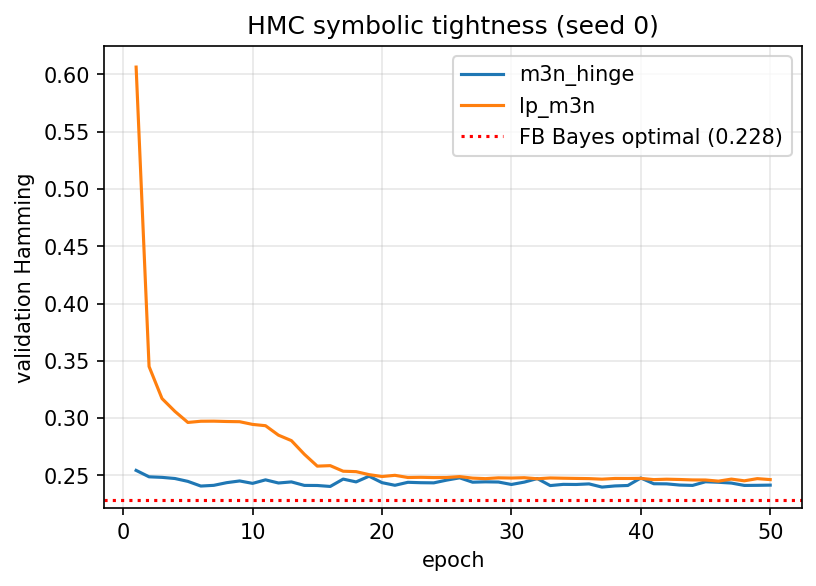
\includegraphics[width=0.7\textwidth]{figures/hmc_sym_tightness/tightness}
\caption[Symbolic HMC convergence curves]{Validation Hamming
versus training epoch on symbolic HMC (seed $0$). Both
M\textsuperscript{3}N losses converge to the same plateau just
above the Forward-Backward Bayes-optimal floor.}
\label{fig:tightness-symbolic-curves}
\end{figure}

\paragraph{Learned pairwise weights.}
Figure~\ref{fig:tightness-symbolic-weights} compares the
learned pairwise matrix $W$ for both losses on seed $0$. Both
methods learn a diagonal-dominant structure, consistent with
$p_{\mathrm{self}} = 0.7$. The Pearson correlation between the
two learned pairwise matrices is $0.92$ (and $0.95$ between the
two backbones' linear weights): the two methods recover
essentially the same model modulo a multiplicative scale.

\begin{figure}[htbp]
\centering
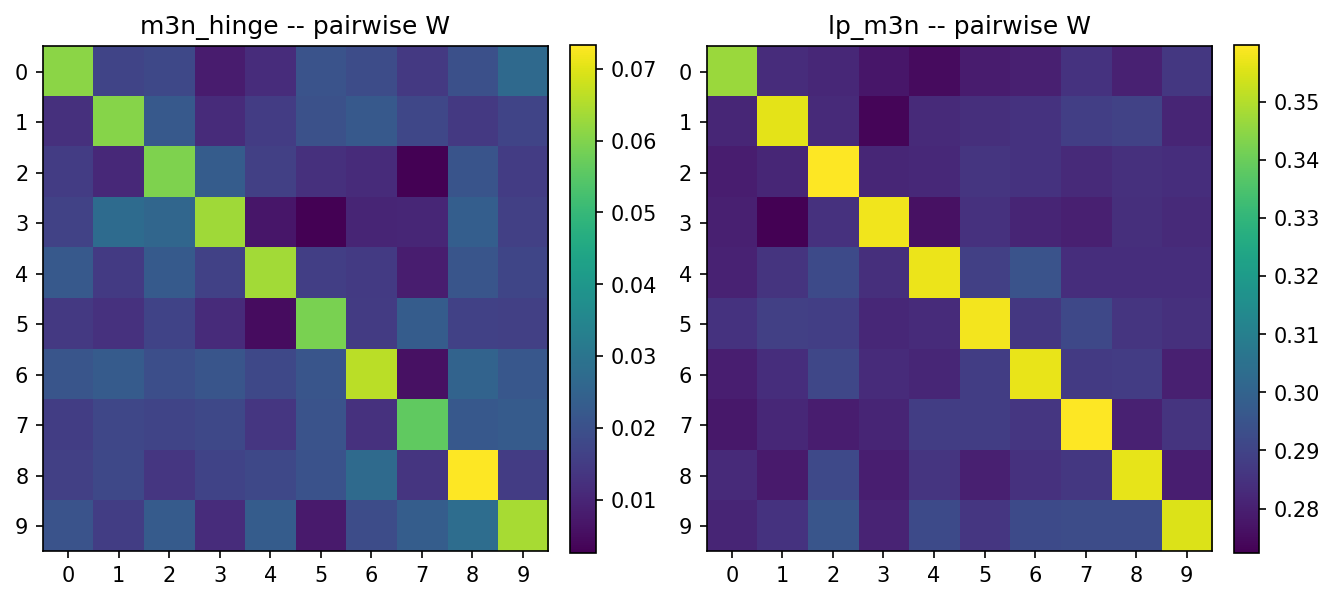
\includegraphics[width=0.95\textwidth]{figures/hmc_sym_tightness/learned_weights}
\caption[Symbolic HMC learned pairwise weights]{Pairwise matrix
$W$ learned by each loss on symbolic HMC (seed $0$). Both
methods recover a diagonal-dominant structure; the structured-hinge
matrix has smaller absolute magnitude but the relative ordering of
entries matches LP-M3N's (Pearson $r = 0.92$).}
\label{fig:tightness-symbolic-weights}
\end{figure}

\subsection{Visual HMC}
\label{subsec:experiments-tightness-visual}

\paragraph{Setup.}
The same chain benchmark as
Section~\ref{subsec:experiments-tightness-symbolic}, but the
observation digits are rendered as MNIST images
(Section~\ref{subsec:hmc-variants}), and the predictor uses
the LeNet-5 backbone of
Section~\ref{subsec:method-architecture-backbones} in place of
the linear baseline. Each loss is run with three seeds at six
values of the regularization strength
$\lambda \in \{0, 10^{-4}, 5\cdot 10^{-4}, 10^{-3}, 5\cdot
10^{-3}, 10^{-2}\}$, giving $36$ runs in total. Training runs
for $200$ epochs.

\paragraph{Best-$\lambda$ results.}
Each loss was run with three seeds at six values of the
regularization strength
$\lambda \in \{0, 10^{-4}, 5\cdot 10^{-4}, 10^{-3}, 5\cdot
10^{-3}, 10^{-2}\}$. Test Hamming was largely insensitive to
$\lambda$ for both losses (variation within $\sim 0.007$). The
best configurations were $\lambda = 5 \cdot 10^{-4}$ for
structured-hinge (test Hamming $0.248 \pm 0.001$) and
$\lambda = 5 \cdot 10^{-3}$ for LP-M3N ($0.246 \pm 0.000$).
Both remain within $0.020$ of the Bayes-optimal floor of
$0.228$; the relaxation tightness is preserved with the
non-linear backbone.

\paragraph{Convergence and overfitting.}
Figure~\ref{fig:tightness-visual-curves} overlays the per-epoch
validation Hamming for the best-$\lambda$ run of each loss on
seed $0$. Both reach the plateau within the first $\sim 50$
epochs. The structured-hinge curve then drifts upward after
epoch $\sim 75$ --- a clear sign of overfitting on the LeNet-5
backbone. LP-M3N stays at the lower plateau through the full
$200$-epoch run, supporting the regularization interpretation
above.

\begin{figure}[htbp]
\centering
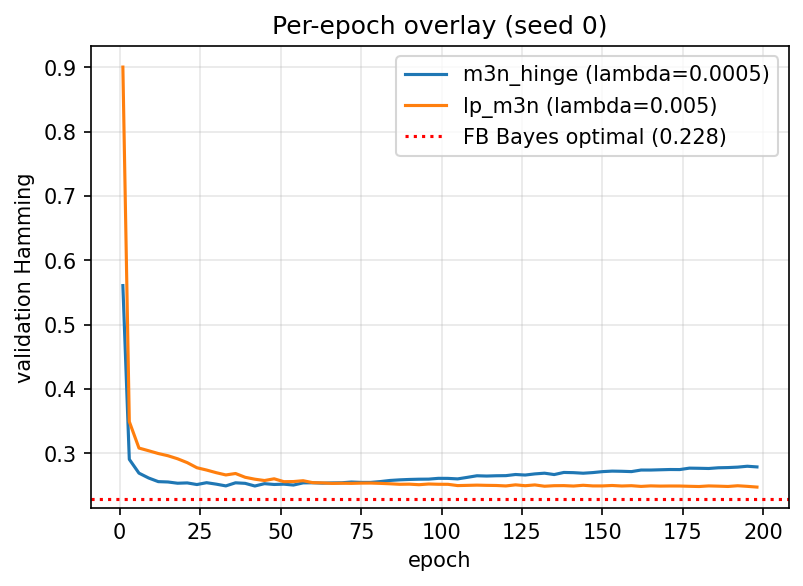
\includegraphics[width=0.75\textwidth]{figures/hmc_vis_tightness/per_epoch}
\caption[Visual HMC convergence curves]{Per-epoch validation
Hamming on visual HMC for the best $\lambda$ per loss (seed
$0$). Structured-hinge overfits the LeNet-5 backbone after
$\sim 75$ epochs; LP-M3N stays at the plateau.}
\label{fig:tightness-visual-curves}
\end{figure}

\paragraph{Learned pairwise weights.}
Figure~\ref{fig:tightness-visual-weights} shows the pairwise
matrix $W$ for the best-$\lambda$ run of each loss on seed
$0$. As in the symbolic case, both methods learn a
diagonal-dominant $W$ with similar relative structure.

\begin{figure}[htbp]
\centering

\includegraphics[width=0.95\textwidth]{figures/hmc_vis_tightness/learned_weights}
\caption[Visual HMC learned pairwise weights]{Learned pairwise
matrix $W$ at the best $\lambda$ per loss on visual HMC
(seed $0$). Both methods recover a diagonal-dominant
structure.}
\label{fig:tightness-visual-weights}
\end{figure}

\subsection{Conclusion}
\label{subsec:experiments-tightness-conclusion}

The LP-relaxed M\textsuperscript{3}N learning loss recovers
test-time performance and learned parameters that are
indistinguishable from exact structured-hinge training on the
linear-chain HMC benchmark, both with the simple linear backbone
and with the LeNet-5 convolutional backbone. The tightness
prediction of Section~\ref{subsec:lp-relaxation} holds
empirically, and the batched LP-M3N implementation is validated
as a correct alternative training path on tree-structured
graphs. With the relaxation validated as a learning device, the
remainder of the chapter applies it to the cyclic Sudoku graph,
where exact training is intractable.
